\chapter{Partitioned Element Methods} \label{ch:pem}
%
This chapter defines a general class of polytopal element formulations, herein referred to as partitioned element methods (PEM). The essential mathematical requirements placed upon these methods are formally stated, giving rise to a family of different approaches, for which some formal investigations are conducted. Several specific formulations are summarized in detail, and a number of existing methods are herein classified as partitioned element methods.

\section{Overview}

A partitioned element method is a finite element-like method which approaches the task of constructing shape functions on an arbitrary element domain by partitioning the element into simpler sub-domains, and establishing a finite sub-space of approximating functions defined on this partition. Optimal shape functions are selected from this approximation space which minimize a chosen objective functional, while respecting any imposed constraints.

The rationale behind this paradigm stems from the idea that it is generally easier to define shape functions which preserve desirable characteristics over arbitrary polytopal domains if the shape functions are defined in a piece-wise polynomial fashion over simpler sub-domains.

Partitioned element methods encompass the special case where each element consists of a single sub-domain, thereby reducing the method to a VEM or VETFEM-like approach. Such methods typically require more rigorous mesh regularity requirements be satisfied to obtain favorable results, however. These approaches are not particularly robust when applied to arbitrary polyhedral meshes, namely those generated by B-rep intersection, and they perform poorly if the element's geometry is sufficiently complicated.

At a minimum, the partitioned element method must satisfy 4 primary conditions:
\begin{itemize}
	\item \textbf{Reproducibility}: The shape functions (and their derivatives) must be capable of exactly reproducing any polynomial field up to a specified order $k$.
	\item \textbf{Compatibility}: The shape functions must maintain a sufficient degree of continuity at inter-element and intra-element interfaces.
	\item \textbf{Stability}: The local bilinear form defined on the element must satisfy the inf-sup condition.
	\item \textbf{Consistency}: The element must exactly integrate the weak form equations when the solution corresponds to a polynomial of maximal degree $k$.
\end{itemize}

In the following sections, an abstract framework for the PEM is established, and the above conditions are made precise in mathematical terms.

\section{An Abstract Partitioned Element Framework}
\subsection{The Element Partition}

\begin{figure} [!ht]
	\centering
	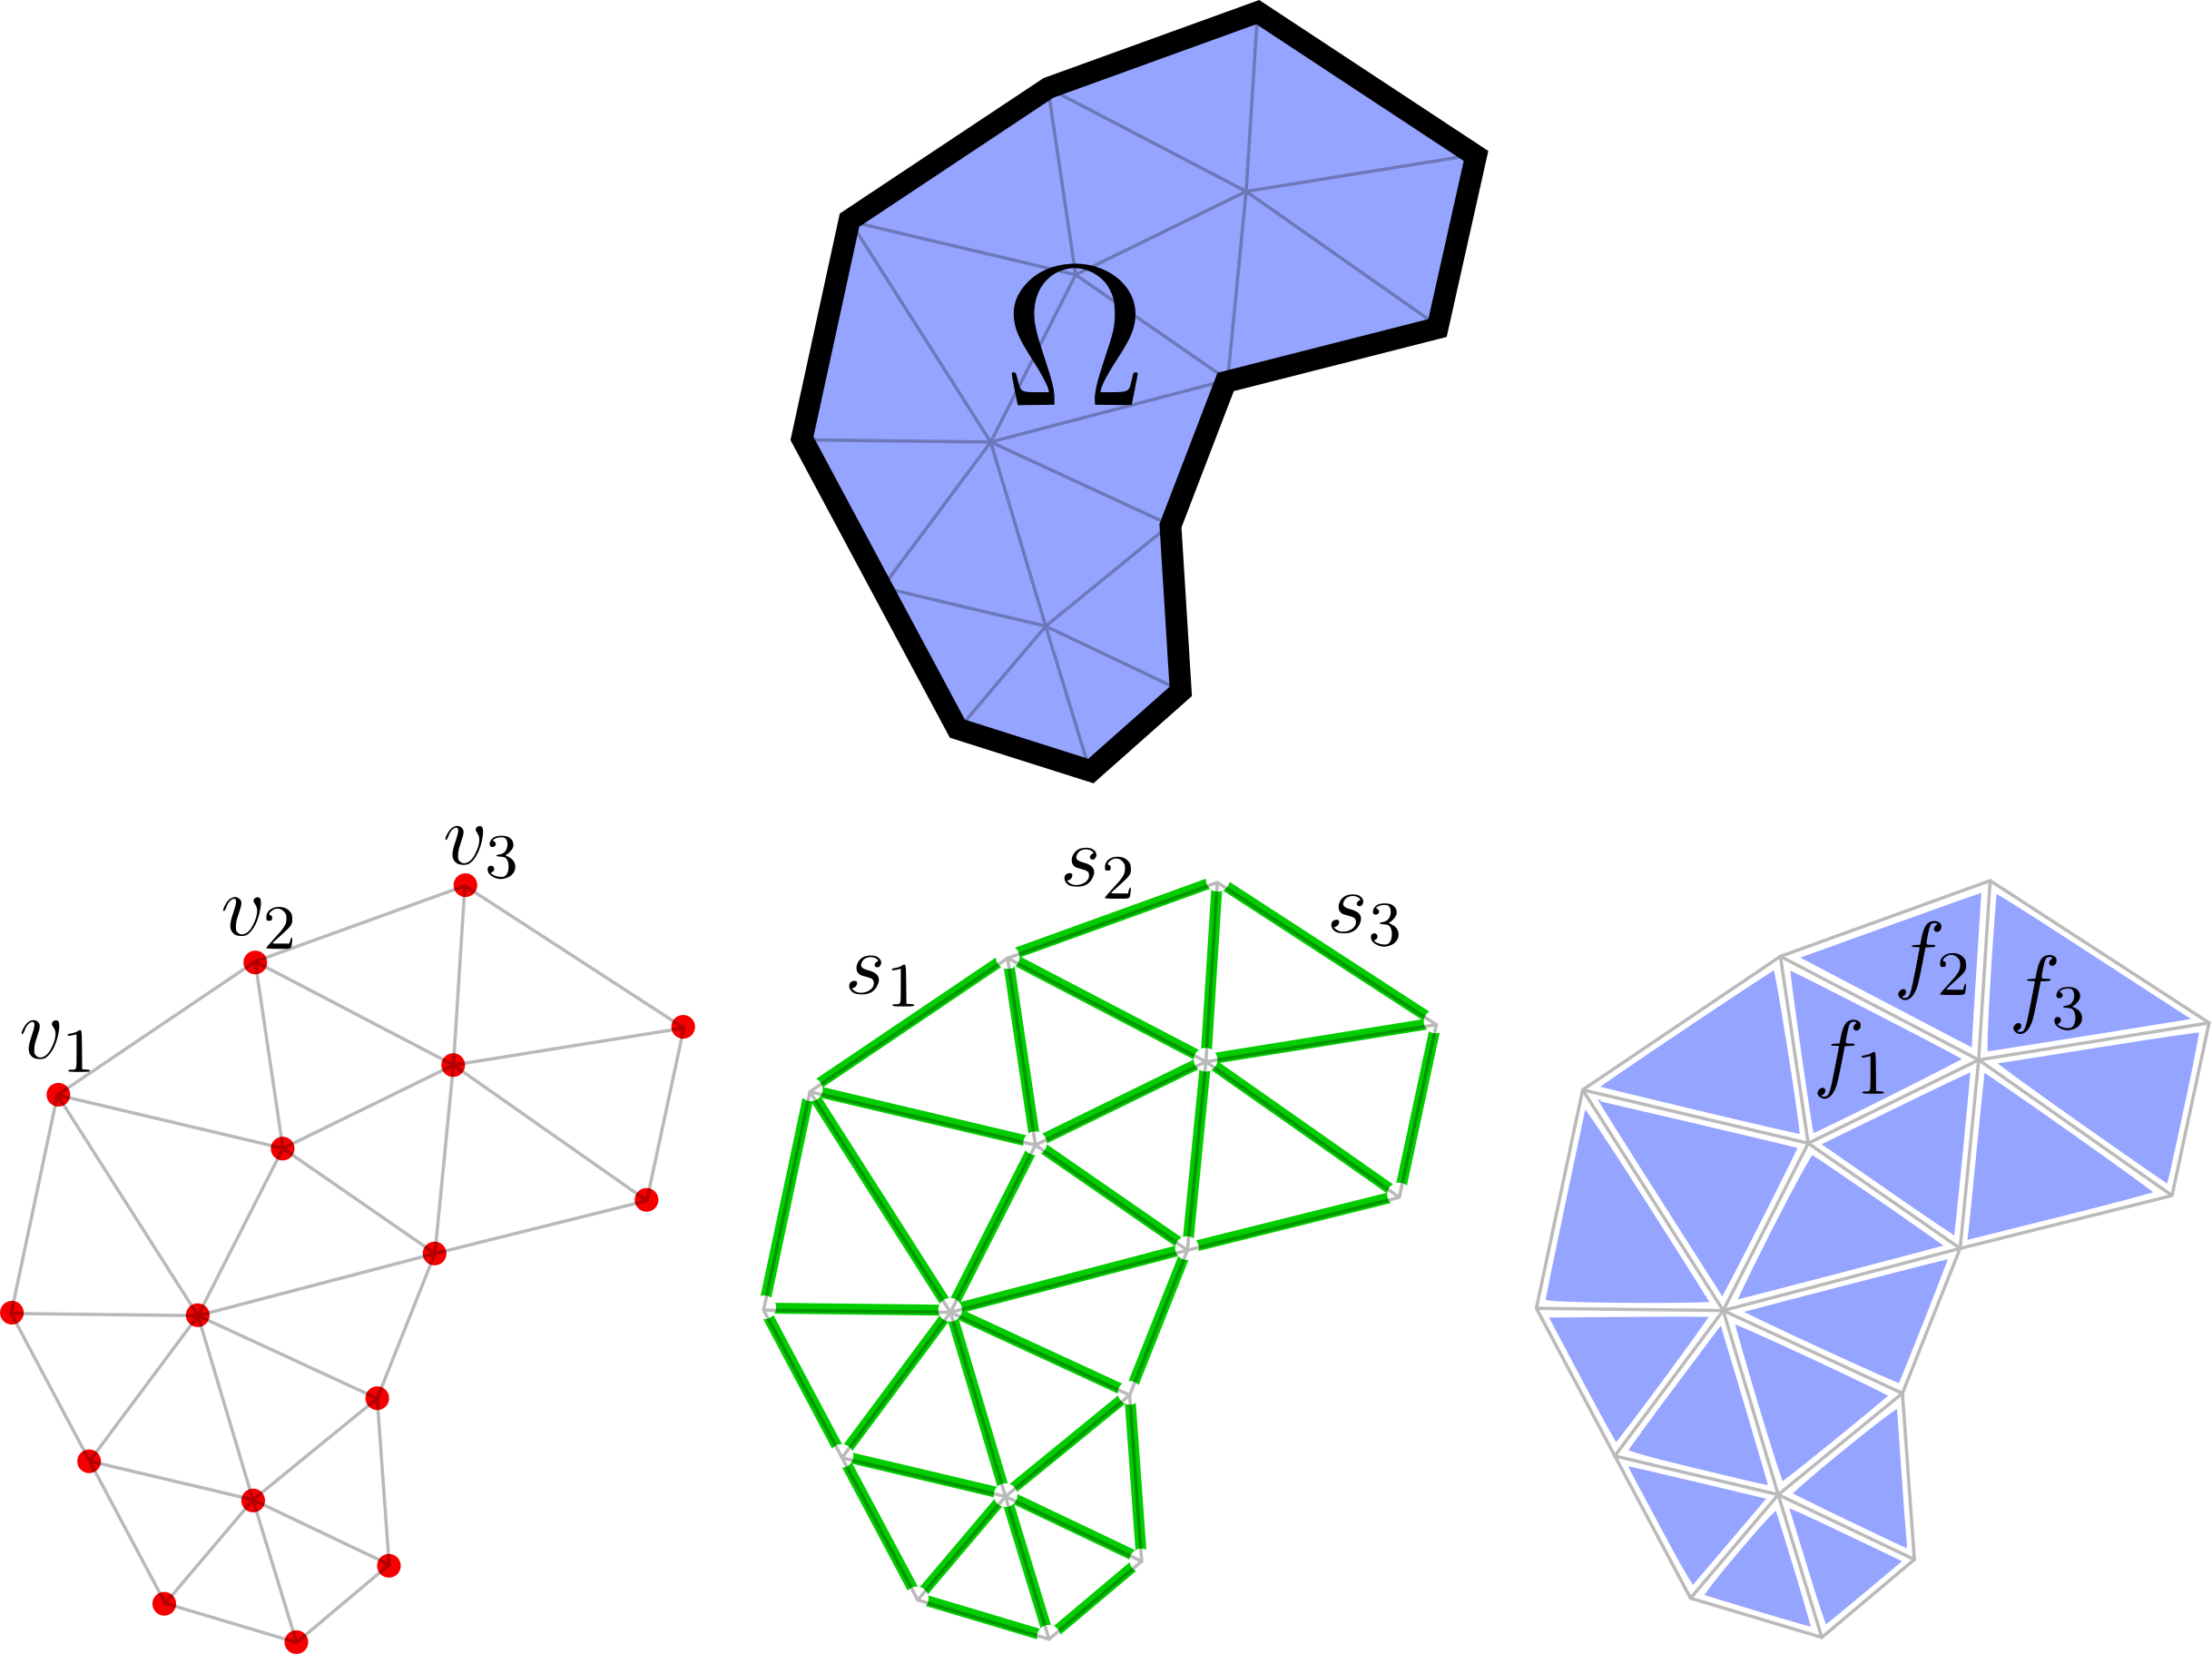
\includegraphics[width = 4.0in]{figures/partition.png}
	\caption{A representative domain $\Omega \subset \mathbb{R}^2$, and it's corresponding partition into verticies, segments, and facets.}
	\label{fig:partitioned_element}
\end{figure}

\begin{itemize}
	\item Provide a figure of an element with partitioned geometry
	\item Define partitioned geometry terms (cells, facets, segments, verticies, etc.), perhaps even give a table of definitions, all referring back to the main figure(s)
	\item 
\end{itemize}

\subsection{Partition-Based Approximation Spaces}

Traditional approximation methods typically consider the independent specification of two principal transformations: an interpolation scheme, which is necessary to represent field variables according to known point-values; and a quadrature rule, for the purposes of integrating such fields over the domain on which they are defined.

In mathematical terms, an interpolant $\varphi$ is a linear operator which maps vectors $\mathbf{u} \in \mathbb{R}^k$ containing point-wise data regarding a field into scalar functions $f \in V^k (\Omega)$, i.e.
\begin{equation}
  \varphi \colon \mathbb{R}^k \mapsto V^k (\Omega)
\end{equation}
where $\mathbb{R}^k$ is a $k$-dimensional real space, and $V^k (\Omega)$ is a $k$-dimensional function space defined on $\Omega$.

By constrast, a quadrature rule $\Sigma$ is a linear operator which maps scalar functions $f \in V^k (\Omega)$ to vectors $\mathbf{q} \in \mathbb{R}^p$ identifying point-wise samples of $f$, i.e.
\begin{equation}
  \Sigma \colon V^k (\Omega) \mapsto \mathbb{R}^p
\end{equation}

The composition $\Sigma \circ \varphi$ of an interpolant $\varphi$ with a quadrature rule $\Sigma$ yields a linear operator
\begin{equation}
  \Sigma \circ \varphi \colon \mathbb{R}^k \mapsto \mathbb{R}^p
\end{equation}

\subsection{Selection of an Appropriate Objective Functional}

Once we have specified a given approximation space of functions, our goal is then to select the function from this space which best represents the nodal data that we are attempting to interpolate over the element. The essential question is this: by what metric should we objectively assess the appropriateness of a given approximating function?

\subsection{Construction of Element Appoximants}

\section{Essential Requirements of the PEM}
\subsection{Reproducibility}

Fundamentally, the approximation power of the PEM depends directly upon the degree of completeness of the underlying approximation space. In particular, the finite-dimensional trial solution space $\mathcal{S}^h$ should contain as a subspace $\mathbb{P}_k \subset \mathcal{S}^h$ for some $k \geq 0$, where $\mathbb{P}_k$ denotes the subspace of polynomial functions with maximal degree $k$. This guarantees that the PEM approximation space will be capable of exactly reproducing any polynomial function up to some specified order.

\subsubsection{Requirements of the Approximation Space}
\subsection{Compatibility}

Compatibility, in an abstract sense, refers to the property of there being a unique displacement field (up to rigid translations) which gives rise to a particular strain field. This condition is satisfied directly if the displacement field is continuous (i.e. if the displacement field $\mathbf{u} \in C^0$). This condition is met if standard ``compatible'' finite elements are utilized, whose trial solution space $\mathcal{S}^h$ is a subset of $C^0$, namely $\mathcal{S}^h \subset H^1 \subset C^0$.

Failure to satisfy compatibility in a strong sense (i.e. point-wise) does not altogether preclude the convergence of a given approximation method. Some authors have proposed that satisfaction of the Irons patch test is sufficient for convergence. It was later shown, however, that the Irons patch test is neither sufficient, nor necessary for convergence. Most notably, Stummel has proposed in \cite{Stummel:79} the necessary and sufficient conditions for convergence of a non-conforming finite element method. These conditions include approximability, and passage of a so-called ``generalized patch test,'' which asserts:

\textit{For a given patch $S \subset \overline{\Omega}$ and an approximating sequence of functions $u^h \in H^k (\Omega^h)$: for every $\mathbf{x} \in S$ there exists an open neighborhood $O$ in $\mathbb{R}^d$ such that}
\begin{equation}
  \lim_{h \rightarrow 0} \sum_{\Omega_e \in \mathcal{P}_h} \int_{\partial \Omega_e} \varphi \, \partial^\alpha u^h|_{\Omega_e} \mathbf{n} \, da = \mathbf{0}
\end{equation}
\textit{for all test functions $\varphi \in C^{\infty}_0 (O)$, and $| \alpha | \leq k-1$.}

Moreover, Stummel provides in \cite{Stummel:80} a number of counter-examples of elements which pass the patch tests of Irons and Strang, but which yield approximations which do not converge to the exact solution.

\subsubsection{Weak Enforcement of Continuity}
\subsection{Stability}
\subsubsection{Restrictions on the Element Partition}
\subsection{Variational Consistency}
\subsubsection{Weak Enforcement of Consistency}

Consider the variational formulation for the model solid mechanics problem:

Find $\mathbf{u} \in \mathcal{S} = \left\{ \mathbf{u} \in H^1(\Omega), \mathbf{u} = \bar{\mathbf{u}} \, \, \forall \mathbf{x} \in \Gamma_u \right\}$ such that
\begin{equation}
  \int_\Omega (T_{ij,j} + \rho b_i) v_i \, dv = 0
\end{equation}
for all $\mathbf{v} \in \mathcal{V} = \left\{ \mathbf{v} \in H^1(\Omega), \mathbf{v} = \mathbf{0} \, \, \forall \mathbf{x} \in \Gamma_u \right\}$. Alternatively,
\begin{equation}
  \int_\Omega T_{ij} v_{i,j} \, dv - \int_\Omega \rho b_i v_i \, dv = \int_{\Gamma_t} \bar{t}_i v_i \, da.
\end{equation}
Now, let us contemplate a particular representation $v^h_i = \sum_{a=1}^N \varphi_a v_{ia}$, where $\mathbf{v}^h \in \mathcal{V}^h$ and $\mathcal{V}^h \subset \mathcal{V}$, resulting in
\begin{equation}
  \int_\Omega T_{ij} \varphi_{a,j} \, dv - \int_\Omega \rho b_i \varphi_a \, dv = \int_{\Gamma_t} \bar{t}_i \varphi_a \, da \quad \forall i, a.
\end{equation}
The above expression should be satisfied \textit{exactly} when the exact solution $\mathbf{u}$ lies within the finite dimensional approximation space $\mathcal{S}^h \subset \mathcal{S}$. Given an exact solution $\bar{T}_{ij}$ arising from some prescribed $\bar{t}_i = \bar{T}_{ij} n_j$ and $\rho b_i = - \bar{T}_{ij,j}$, we may express
\begin{equation}
  \int_\Omega \bar{T}_{ij} \varphi_{a,j} \, dv + \int_\Omega \bar{T}_{ij,j} \varphi_a \, dv = \int_{\partial \Omega} \bar{T}_{ij} n_j \varphi_a \, da \quad \forall i, a.
\end{equation}
If $\bar{T}_{ij}$ can be written as a polynomial expansion, i.e.
\begin{equation}
  \bar{T}_{ij} (\mathbf{x}) = \sum_{|\alpha| = 0}^k \bar{T}_{ij\alpha} \mathbf{x}^\alpha,
\end{equation}
then the $\alpha$-th order variational consistency requirement asserts:
\begin{equation}
  \int_\Omega \mathbf{x}^{\alpha} \varphi_{a,i} \, dv + \int_\Omega \mathbf{x}^{\alpha}_{,i} \varphi_a \, dv = \int_{\partial \Omega} \mathbf{x}^{\alpha} n_i \varphi_a \, da \quad \forall i, a.
\end{equation}
This degree of consistency is required if the bi-linear form $B(u,v)$ on $\mathcal{S}$ and $\mathcal{V}$ is to determine uniqueness of any exact polynomial solutions contained within $\mathcal{S}$. Moreover, the above expression guarantees that any solution may be reasonably well approximated by low-order polynomials in the locality of the selected domain $\Omega$.

Consequently, we may consider an application of the above consistency requirements to the entire problem domain $\Omega$, or -- more practically -- we may enforce consistency up to the desired order on each element domain $\Omega_e$. The element-local $\alpha$-th order consistency equations follow:
\begin{equation}
  \int_{\Omega_e} \mathbf{x}^{\alpha} \varphi_{a,i} \, dv + \int_{\Omega_e} \mathbf{x}^{\alpha}_{,i} \varphi_a \, dv = \int_{\partial \Omega_e} \mathbf{x}^{\alpha} n_i \varphi_a \, da \quad \forall i, a.
  \label{eq:consistency}
\end{equation}

It should be emphasized that the consistency equations set forth are conditions which apply only to the test functions $\varphi_a \in \mathcal{V}^h$, and not to the trial functions $\phi_a \in \mathcal{S}^h$. The trial solution space must, however, be capable of reproducing all polynomial solutions (and their derivatives) up to some corresponding order $k$, such that $\mathbb{P}_k \subset \mathcal{S}^h$.

In most practical situations, it may not be possible to evaluate the integral expressions exactly. Instead, numerical quadrature rules must be defined, both on the element's interior, and on its boundary, such that
\begin{equation}
  \int_{\Omega_e} f(\mathbf{x}) dv \approx \sum_{q=1}^{N_q} w_q f(\mathbf{x}_q),
\end{equation}
\begin{equation}
  \int_{\partial \Omega_e} f(\mathbf{x}) da \approx \sum_{b=1}^{N_b} w_b f(\mathbf{x}_b).
\end{equation}
This yields yet another form of consistency, henceforth referred to as ``quadrature consistency,'' expressed as:
\begin{equation}
  \sum_{q=1}^{N_q} w_q \left[ \mathbf{x}_q^{\alpha} \varphi^{(q)}_{a,i} + \mathbf{x}^{\alpha}_{q,i} \varphi^{(q)}_a \right] = \sum_{b=1}^{N_b} w_b \mathbf{x}_b^{\alpha} n^{(b)}_i \varphi^{(b)}_a \quad \forall i, a.
  \label{eq:quadrature_consistency}
\end{equation}
Moving forward in our developments, quadrature consistency will be the only form of consistency of practical interest, as it appropriately reflects the discrete data quantities at our disposal.

A brief remark should be made regarding the lack of equivalence between the exact evaluation of consistency in equation (\ref{eq:consistency}) and its numerical approximation in equation (\ref{eq:quadrature_consistency}). In general, we cannot claim that satisfaction of one guarantees the other. There is only one occasion when we may say that (\ref{eq:quadrature_consistency}) holds if and only if (\ref{eq:consistency}) is satisfied, which occurs only when sufficiently accurate quadrature rules are used on the element and its boundary. In the vast majority of situations, however, this is an impractical constraint, as the construction of high-order quadrature rules on arbitrary polyhedra (though possible) proves to be somewhat computationally intensive (see the literature by Sukumar, etc.). Moreover, without a precise representation of the test functions over the element domain, it becomes infeasible to consider an exact integration of such functions.

\subsection{Numerical Quadrature Consistency}

Beyond consistency with the weak form for a specified subspace of polynomial functions used to represent the solution, we also require that the numerical quadrature scheme utilized be sufficiently accurate to the extent that: Galerkin exactness is satisfied for certain classes of solutions, and that the quadrature error has a bound which is of a lower order than that of the approximation error.

\subsubsection{Bubnov-Galerkin and Petrov-Galerkin Approaches}

\section{Specific Formulations}
\subsection{The Continuous-Galerkin PEM}
\subsection{The Weak-Galerkin PEM}
\subsection{The Discontinuous-Galerkin PEM}

\section{Enhancements to Improve Solution Accuracy}
\subsection{Partition-Based Enhancement Functions}
\subsection{Mixed PEM Discretizations}
